\documentclass[tikz,border=12pt]{standalone}
\usepackage{amsmath}
\usetikzlibrary{arrows.meta}
\definecolor{field}{RGB}{45,95,160}
\definecolor{particle}{RGB}{185,60,40}
\definecolor{observer}{RGB}{40,130,105}
\begin{document}
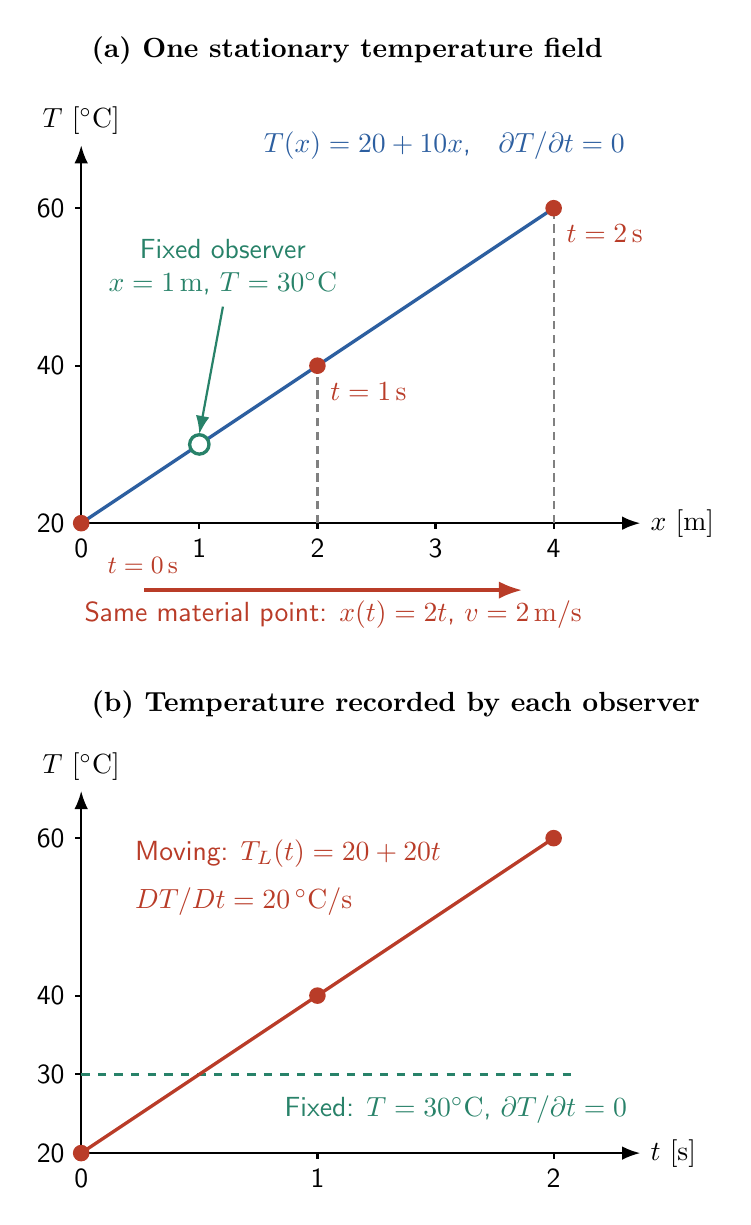
\begin{tikzpicture}[>=Latex,font=\sffamily,thick]
% Vertical coordinates represent (T - 20 deg C) / 10.
\node[anchor=west,font=\bfseries] at (0,6.0) {(a) One stationary temperature field};
\draw[->] (0,0)--(7.1,0) node[right] {$x\ [\mathrm m]$};
\draw[->] (0,0)--(0,4.8) node[above] {$T\ [^\circ\mathrm C]$};
\foreach \x in {0,1,2,3,4} {
  \draw (1.5*\x,0)--(1.5*\x,-0.08);
  \node[below] at (1.5*\x,-0.08) {\x};
}
\foreach \y/\temp in {0/20,2/40,4/60} {
  \draw (0,\y)--(-0.08,\y);
  \node[left] at (-0.08,\y) {\temp};
}
\draw[field,very thick] (0,0)--(6,4);
\node[field,anchor=west,fill=white,inner sep=3pt] at (2.2,4.8)
  {$T(x)=20+10x$,\quad $\partial T/\partial t=0$};
\foreach \x/\y/\time in {0/0/0,3/2/1,6/4/2} {
  \draw[densely dashed,gray] (\x,0)--(\x,\y);
  \fill[particle] (\x,\y) circle (3pt);
  \ifnum\time>0
    \node[particle,anchor=north west,fill=white,inner sep=2pt] at (\x+0.08,\y-0.13)
      {$t=\time\,\mathrm s$};
  \fi
}
\node[particle,anchor=north west,font=\small,inner sep=2pt] at (0.25,-0.35) {$t=0\,\mathrm s$};
\draw[observer,fill=white,very thick] (1.5,1) circle (3.5pt);
\draw[observer,->] (1.8,2.75)--(1.5,1.13);
\node[observer,align=center] at (1.8,3.25) {Fixed observer\\$x=1\,\mathrm m$, $T=30^\circ\mathrm C$};
\draw[particle,->,very thick] (0.8,-0.85)--(5.6,-0.85)
  node[midway,below] {Same material point: $x(t)=2t$, $v=2\,\mathrm{m/s}$};

\begin{scope}[shift={(0,-8.0)}]
  \node[anchor=west,font=\bfseries] at (0,5.7) {(b) Temperature recorded by each observer};
  \draw[->] (0,0)--(7.1,0) node[right] {$t\ [\mathrm s]$};
  \draw[->] (0,0)--(0,4.6) node[above] {$T\ [^\circ\mathrm C]$};
  \foreach \x/\time in {0/0,3/1,6/2} {
    \draw (\x,0)--(\x,-0.08);
    \node[below] at (\x,-0.08) {\time};
  }
  \foreach \y/\temp in {0/20,1/30,2/40,4/60} {
    \draw (0,\y)--(-0.08,\y);
    \node[left] at (-0.08,\y) {\temp};
  }
  \draw[observer,dashed,very thick] (0,1)--(6.3,1);
  \node[observer,anchor=west,fill=white,inner sep=2pt] at (2.5,0.55)
    {Fixed: $T=30^\circ\mathrm C$, $\partial T/\partial t=0$};
  \draw[particle,very thick] (0,0)--(6,4);
  \foreach \x/\y in {0/0,3/2,6/4} {\fill[particle] (\x,\y) circle (3pt);}
  \node[particle,anchor=west,fill=white,inner sep=2pt] at (0.6,3.8)
    {Moving: $T_L(t)=20+20t$};
  \node[particle,anchor=west,fill=white,inner sep=2pt] at (0.6,3.2)
    {$DT/Dt=20\,{}^\circ\mathrm C/\mathrm s$};
\end{scope}
\end{tikzpicture}
\end{document}
